% \documentclass{article}
% \usepackage{graphicx}

% \title{Conceptual Dependencies}
% \begin{document}
    % \maketitle

    Conceptual Dependency (CD) theory~\cite{SCHANK1972552} is a method of expressing meaning, rather than syntax. It is based on the notion of expressing concepts in terms of basic physical notions- either literally, when describing physical events, or metaphorically, when describing abstract exchanges (of value or information). As CD is syntax independent, it can be applied to any language or similar information encoding.

    CD expresses events in terms of a number of predefined primitives. Some of the physical primitives defined by Schank are:
    \begin{itemize}
        \item \textbf{PTRANS}- an entity's physical location changing
        \item \textbf{MOVE}- a object moving a part of itself (e.g.~a person moving their arm)
        \item \textbf{PROPEL}- an entity applying a force to another object
        \item \textbf{EMIT}- an entity ejecting another object from inside itself
        \item \textbf{INJECT}- an entity taking another object into itself
    \end{itemize}

    The more abstract primitives include:
    \begin{itemize}
        \item \textbf{MTRANS}- transferring information between two concious entities
        \item \textbf{ATRANS}- altering an abstract property (e.g.~ownership of an entity)
    \end{itemize}

    Other parameters to a scenario can be expressed using Schank's system:
    \begin{itemize}
        \item The object of an action (in a grammatical sense), designated with \emph{o}
        \item The direction in which a change is made, designated with \emph{D}
        \item The recipient of a change, designated with \emph{R}
        \item One scenario can result in another one, designated with lower case \emph{r}
    \end{itemize}

    Schank devised a system of diagrams for expressing scenarios in terms of their conceptual Dependencies, which will be used in this dissertation. Figure~\ref{fig:emit-cd} shows the verb `emit' expressed as a CD diagram.
    \begin{figure}
        \centerline{
            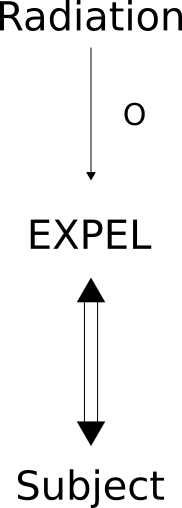
\includegraphics[height=200pt]{diagrams/emit-cd.png}
        }
        \caption{A CD diagram of the verb `emit'. As something is being taken from inside the subject and forced out, it corresponds to the `Expel' primitive in CD.\@The `object' of this verb is radiation of some sort.}
        \label{fig:emit-cd}
    \end{figure}


    \bibliographystyle{plain}
    \bibliography{refs}
% \end{document}